\documentclass{standalone}
\usepackage{tikz}
\usetikzlibrary{patterns, positioning}


\begin{document}
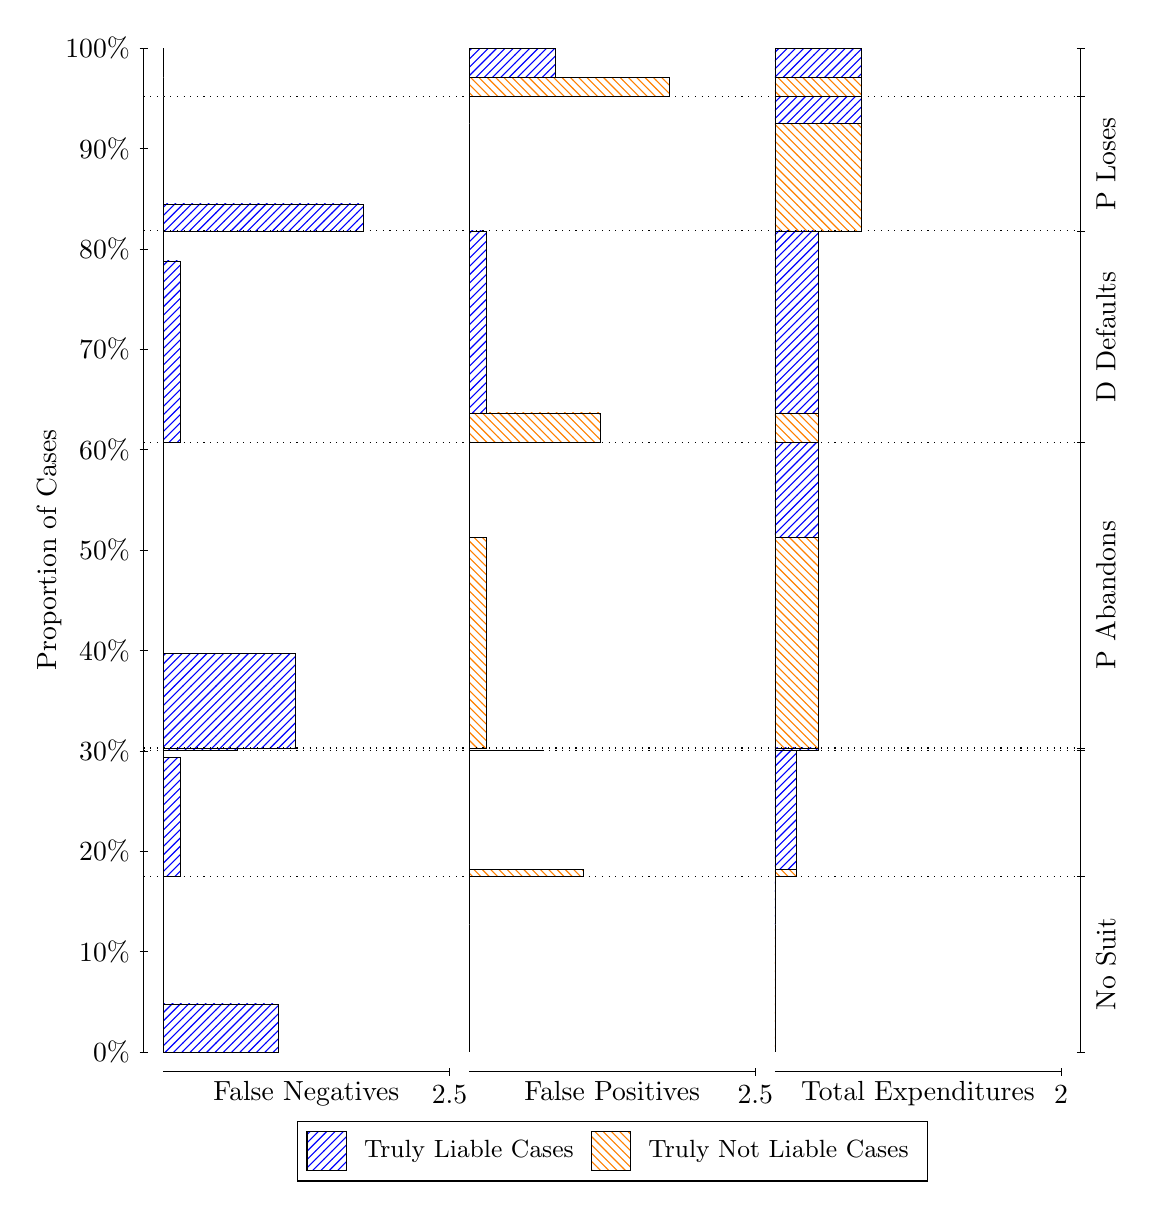
\begin{tikzpicture}
\draw[black, very thin] (1.5,1.75) -- (1.5,14.5);
\node[rotate=90, text=black, anchor=center] at (0.3, 8.125) {Proportion of Cases};
\draw[black, very thin] (1.45,1.75) -- (1.55,1.75);
\node[text=black, anchor=east] at (1.45, 1.75) {0\%};
\draw[black, very thin] (1.45,3.025) -- (1.55,3.025);
\node[text=black, anchor=east] at (1.45, 3.025) {10\%};
\draw[black, very thin] (1.45,4.3) -- (1.55,4.3);
\node[text=black, anchor=east] at (1.45, 4.3) {20\%};
\draw[black, very thin] (1.45,5.575) -- (1.55,5.575);
\node[text=black, anchor=east] at (1.45, 5.575) {30\%};
\draw[black, very thin] (1.45,6.85) -- (1.55,6.85);
\node[text=black, anchor=east] at (1.45, 6.85) {40\%};
\draw[black, very thin] (1.45,8.125) -- (1.55,8.125);
\node[text=black, anchor=east] at (1.45, 8.125) {50\%};
\draw[black, very thin] (1.45,9.4) -- (1.55,9.4);
\node[text=black, anchor=east] at (1.45, 9.4) {60\%};
\draw[black, very thin] (1.45,10.675) -- (1.55,10.675);
\node[text=black, anchor=east] at (1.45, 10.675) {70\%};
\draw[black, very thin] (1.45,11.95) -- (1.55,11.95);
\node[text=black, anchor=east] at (1.45, 11.95) {80\%};
\draw[black, very thin] (1.45,13.225) -- (1.55,13.225);
\node[text=black, anchor=east] at (1.45, 13.225) {90\%};
\draw[black, very thin] (1.45,14.5) -- (1.55,14.5);
\node[text=black, anchor=east] at (1.45, 14.5) {100\%};

\draw[black, very thin] (13.4,1.75) -- (13.4,14.5);
\draw[black, very thin] (13.35,1.75) -- (13.45,1.75);
\node[anchor=west] at (13.35, 1.75) {};
\draw[black, very thin] (13.35,3.9791) -- (13.45,3.9791);
\node[anchor=west] at (13.35, 3.9791) {};
\draw[black, very thin] (13.35,5.5817) -- (13.45,5.5817);
\node[anchor=west] at (13.35, 5.5817) {};
\draw[black, very thin] (13.35,5.6106) -- (13.45,5.6106);
\node[anchor=west] at (13.35, 5.6106) {};
\draw[black, very thin] (13.35,9.4878) -- (13.45,9.4878);
\node[anchor=west] at (13.35, 9.4878) {};
\draw[black, very thin] (13.35,12.177) -- (13.45,12.177);
\node[anchor=west] at (13.35, 12.177) {};
\draw[black, very thin] (13.35,13.883) -- (13.45,13.883);
\node[anchor=west] at (13.35, 13.883) {};
\draw[black, very thin] (13.35,14.5) -- (13.45,14.5);
\node[anchor=west] at (13.35, 14.5) {};

\draw[black, very thin, pattern color=blue, pattern=north east lines] (1.75,1.75) rectangle (3.2033,2.3618);
\draw[black, very thin, pattern color=orange, pattern=north west lines] (1.75,2.3618) rectangle (1.75,3.9791);
\draw[black, very thin, pattern color=blue, pattern=north east lines] (1.75,3.9791) rectangle (1.968,5.4889);
\draw[black, very thin, pattern color=orange, pattern=north west lines] (1.75,5.4889) rectangle (1.75,5.5817);
\draw[black, very thin, pattern color=blue, pattern=north east lines] (1.75,5.5817) rectangle (2.6947,5.6087);
\draw[black, very thin, pattern color=orange, pattern=north west lines] (1.75,5.6087) rectangle (1.75,5.6106);
\draw[black, very thin, pattern color=blue, pattern=north east lines] (1.75,5.6106) rectangle (3.4213,6.8089);
\draw[black, very thin, pattern color=orange, pattern=north west lines] (1.75,6.8089) rectangle (1.75,9.4878);
\draw[black, very thin, pattern color=blue, pattern=north east lines] (1.75,9.4878) rectangle (1.968,11.798);
\draw[black, very thin, pattern color=orange, pattern=north west lines] (1.75,11.798) rectangle (1.75,12.177);
\draw[black, very thin, pattern color=blue, pattern=north east lines] (1.75,12.177) rectangle (4.2933,12.521);
\draw[black, very thin, pattern color=orange, pattern=north west lines] (1.75,12.521) rectangle (1.75,13.883);
\draw[black, very thin, pattern color=orange, pattern=north west lines] (1.75,13.883) rectangle (1.75,14.126);
\draw[black, very thin, pattern color=blue, pattern=north east lines] (1.75,14.126) rectangle (1.75,14.5);
\draw[black, very thin, pattern color=orange, pattern=north west lines] (5.6333,1.75) rectangle (5.6333,3.3672);
\draw[black, very thin, pattern color=blue, pattern=north east lines] (5.6333,3.3672) rectangle (5.6333,3.9791);
\draw[black, very thin, pattern color=orange, pattern=north west lines] (5.6333,3.9791) rectangle (7.0867,4.0718);
\draw[black, very thin, pattern color=blue, pattern=north east lines] (5.6333,4.0718) rectangle (5.6333,5.5817);
\draw[black, very thin, pattern color=orange, pattern=north west lines] (5.6333,5.5817) rectangle (6.578,5.5836);
\draw[black, very thin, pattern color=blue, pattern=north east lines] (5.6333,5.5836) rectangle (5.6333,5.6106);
\draw[black, very thin, pattern color=orange, pattern=north west lines] (5.6333,5.6106) rectangle (5.8513,8.2894);
\draw[black, very thin, pattern color=blue, pattern=north east lines] (5.6333,8.2894) rectangle (5.6333,9.4878);
\draw[black, very thin, pattern color=orange, pattern=north west lines] (5.6333,9.4878) rectangle (7.3047,9.8668);
\draw[black, very thin, pattern color=blue, pattern=north east lines] (5.6333,9.8668) rectangle (5.8513,12.177);
\draw[black, very thin, pattern color=orange, pattern=north west lines] (5.6333,12.177) rectangle (5.6333,13.54);
\draw[black, very thin, pattern color=blue, pattern=north east lines] (5.6333,13.54) rectangle (5.6333,13.883);
\draw[black, very thin, pattern color=orange, pattern=north west lines] (5.6333,13.883) rectangle (8.1767,14.126);
\draw[black, very thin, pattern color=blue, pattern=north east lines] (5.6333,14.126) rectangle (6.7233,14.5);
\draw[black, very thin, pattern color=orange, pattern=north west lines] (9.5167,1.75) rectangle (9.5167,3.3672);
\draw[black, very thin, pattern color=blue, pattern=north east lines] (9.5167,3.3672) rectangle (9.5167,3.9791);
\draw[black, very thin, pattern color=orange, pattern=north west lines] (9.5167,3.9791) rectangle (9.7892,4.0718);
\draw[black, very thin, pattern color=blue, pattern=north east lines] (9.5167,4.0718) rectangle (9.7892,5.5817);
\draw[black, very thin, pattern color=orange, pattern=north west lines] (9.5167,5.5817) rectangle (10.062,5.5836);
\draw[black, very thin, pattern color=blue, pattern=north east lines] (9.5167,5.5836) rectangle (10.062,5.6106);
\draw[black, very thin, pattern color=orange, pattern=north west lines] (9.5167,5.6106) rectangle (10.062,8.2894);
\draw[black, very thin, pattern color=blue, pattern=north east lines] (9.5167,8.2894) rectangle (10.062,9.4878);
\draw[black, very thin, pattern color=orange, pattern=north west lines] (9.5167,9.4878) rectangle (10.062,9.8668);
\draw[black, very thin, pattern color=blue, pattern=north east lines] (9.5167,9.8668) rectangle (10.062,12.177);
\draw[black, very thin, pattern color=orange, pattern=north west lines] (9.5167,12.177) rectangle (10.607,13.54);
\draw[black, very thin, pattern color=blue, pattern=north east lines] (9.5167,13.54) rectangle (10.607,13.883);
\draw[black, very thin, pattern color=orange, pattern=north west lines] (9.5167,13.883) rectangle (10.607,14.126);
\draw[black, very thin, pattern color=blue, pattern=north east lines] (9.5167,14.126) rectangle (10.607,14.5);
\draw[black, dotted] (1.5,3.9791) -- (13.4,3.9791);
\draw[black, dotted] (1.5,5.5817) -- (13.4,5.5817);
\draw[black, dotted] (1.5,5.6106) -- (13.4,5.6106);
\draw[black, dotted] (1.5,9.4878) -- (13.4,9.4878);
\draw[black, dotted] (1.5,12.177) -- (13.4,12.177);
\draw[black, dotted] (1.5,13.883) -- (13.4,13.883);
\draw[black, very thin] (1.75,1.5) -- (5.3833,1.5);
\node[text=black, anchor=north] at (3.5667, 1.5) {False Negatives};
\draw[black, very thin] (5.3833,1.45) -- (5.3833,1.55);
\node[text=black, anchor=north] at (5.3833, 1.45) {2.5};

\draw[black, very thin] (5.6333,1.5) -- (9.2667,1.5);
\node[text=black, anchor=north] at (7.45, 1.5) {False Positives};
\draw[black, very thin] (9.2667,1.45) -- (9.2667,1.55);
\node[text=black, anchor=north] at (9.2667, 1.45) {2.5};

\draw[black, very thin] (9.5167,1.5) -- (13.15,1.5);
\node[text=black, anchor=north] at (11.333, 1.5) {Total Expenditures};
\draw[black, very thin] (13.15,1.45) -- (13.15,1.55);
\node[text=black, anchor=north] at (13.15, 1.45) {2};

\node[text=black, centered, rotate=90] at (13.72, 2.8645) {No Suit};


\node[text=black, centered, rotate=90] at (13.72, 7.5492) {P Abandons};
\node[text=black, centered, rotate=90] at (13.72, 10.833) {D Defaults};
\node[text=black, centered, rotate=90] at (13.72, 13.03) {P Loses};


\draw (7.449999999999999,1.5) node[draw=none] (baseCoordinate) {};
\begin{scope}[align=center]
        \matrix[scale=0.5, draw=black, below=0.5cm of baseCoordinate, nodes={draw}, column sep=0.1cm]{
            \node[rectangle, draw, minimum width=0.5cm, minimum height=0.5cm, pattern color=blue, pattern=north east lines] {}; &
            \node[draw=none, font=\small, text=black] (B) {Truly Liable Cases}; &
            \node[rectangle, draw, minimum width=0.5cm, minimum height=0.5cm, pattern color=orange, pattern=north west lines] {}; &
            \node[draw=none, font=\small, text=black] (B) {Truly Not Liable Cases}; \\
            };
\end{scope}

\end{tikzpicture}
\end{document}